\section{Appendix}

\crefalias{section}{appsec}

\subsection{Feature Sets}
\label{app:feature-sets}

\begin{table}[H]
    \centering
    \begin{threeparttable}
    \begin{tabular}{@{}lllllll@{}}
        \toprule
        Feature Name            & Definition                                                                                       & Origin               & FS 1 & FS 2 & FS 3 & Transform     \\ \midrule
        trade price             & $P_{i, t}$                                                                                       & tick rule            & x    & x    & x    & $\log(\cdot)$ \\
        price lag (ex)          & $P_{i, t-1}^{\text{ex}}$\tnote{*}                                                                & tick rule            & x    & x    & x    & $\log(\cdot)$ \\
        price lag (all)         & $P_{i, t-1}^{\text{all}}$\tnote{*}                                                               & tick rule            & x    & x    & x    & $\log(\cdot)$ \\
        price change lag (ex)   & $P_{i, t-1}^{\text{ex}}/P_{i, t}^{\text{ex}}$\tnote{*}                                           & tick rule            & x    & x    & x    &               \\
        price change lag (all)  & $P_{i, t-1}^{\text{all}}/P_{i, t}^{\text{all}}$\tnote{*}                                         & tick rule            & x    & x    & x    &               \\
        priced lead (ex)        & $P_{i, t+1}^{\text{ex}}$\tnote{*}                                                                & rev. tick rule       & x    & x    & x    & $\log(\cdot)$ \\
        price lead (all)        & $P_{i, t+1}^{\text{all}}$\tnote{*}                                                               & rev. tick rule       & x    & x    & x    & $\log(\cdot)$ \\
        price change lead (ex)  & $P_{i, t}^{\text{ex}}/P_{i, t+1}^{\text{ex}}$\tnote{*}                                           & rev. tick rule       & x    & x    & x    &               \\
        price change lead (all) & $P_{i, t}^{\text{all}}/P_{i, t+1}^{\text{all}}$\tnote{*}                                         & rev. tick rule       & x    & x    & x    &               \\
        bid (all)               & $B_{i, t}^{\text{all}}$                                                                          & quote rule           & x    & x    & x    & $\log(\cdot)$ \\
        bid (ex)                & $B_{i, t}^{\text{ex}}$                                                                           & quote rule           & x    & x    & x    & $\log(\cdot)$ \\
        ask (all)               & $A_{i, t}^{\text{all}}$                                                                          & quote rule           & x    & x    & x    & $\log(\cdot)$ \\
        ask (ex)                & $A_{i, t}^{\text{all}}$                                                                          & quote rule           & x    & x    & x    & $\log(\cdot)$ \\
        prox. to quotes (ex)    & $\left(P_{i, t}^{\text{ex}}- M_{i, t}^{\text{ex}}\right) / \tfrac{1}{2} S_{i, t}^{\text{ex}}$    & \gls{EMO}/\gls{CLNV} & x    & x    & x    &               \\
        prox. to quotes (all)   & $\left(P_{i, t}^{\text{all}}- M_{i, t}^{\text{all}}\right) / \tfrac{1}{2} S_{i, t}^{\text{all}}$ & \gls{EMO}/\gls{CLNV} & x    & x    & x    &               \\
        bid ask size ratio (ex) & $\tilde{B}_{i, t}^{\text{ex}}/\tilde{A}_{i, t}^{\text{ex}}$                                      & depth rule           &      & x    & x    &               \\
        bid size (ex)           & $\tilde{B}_{i, t}^{\text{ex}}$                                                                   & depth rule           &      & x    & x    &               \\
        ask size (ex)           & $\tilde{A}_{i, t}^{\text{ex}}$                                                                   & depth rule           &      & x    & x    &               \\
        rel. bid size (ex)      & $\tilde{B}_{i, t}^{\text{ex}}/\tilde{P}_{i, t}^{\text{ex}}$                                      & trade size rule      &      & x    & x    &               \\
        rel. ask size (ex)      & $\tilde{A}_{i, t}^{\text{ex}}/\tilde{P}_{i, t}^{\text{ex}}$                                      & trade size rule      &      & x    & x    &               \\
        trade size              & $\tilde{P}_{i, t}$                                                                               & trade size rule      &      & x    & x    &               \\
        strike price            &                                                                                                  & option               &      &      & x    & $\log(\cdot)$ \\
        volume option series    &                                                                                                  & option               &      &      & x    & $\log(\cdot)$ \\
        root                    &                                                                                                  & option               &      &      & x    & binarize      \\
        time to maturity        &                                                                                                  & option               &      &      & x    &               \\
        moneyness               &                                                                                                  & option               &      &      & x    &               \\
        option type             &                                                                                                  & option               &      &      & x    & binarize      \\
        issue type              &                                                                                                  & option               &      &      & x    & binarize      \\ \bottomrule
    \end{tabular}
    \begin{tablenotes}\footnotesize
        \item[*] Notation assumes, that the previous or next trade price is distinguishable.
    \end{tablenotes}
\end{threeparttable}
    \caption[Overview of Feature Sets]{Definition of Feature Sets}
    \label{tab:feature-set-definition}
\end{table}

\newpage

\newpage
\subsection{Power-Transforms of Features}
\label{app:power-transforms-of-features}

\newpage
\subsection{Autocorrelation of Features}
\label{app:autocorrelation-of-features}

\begin{figure}[ht]
    \centering
    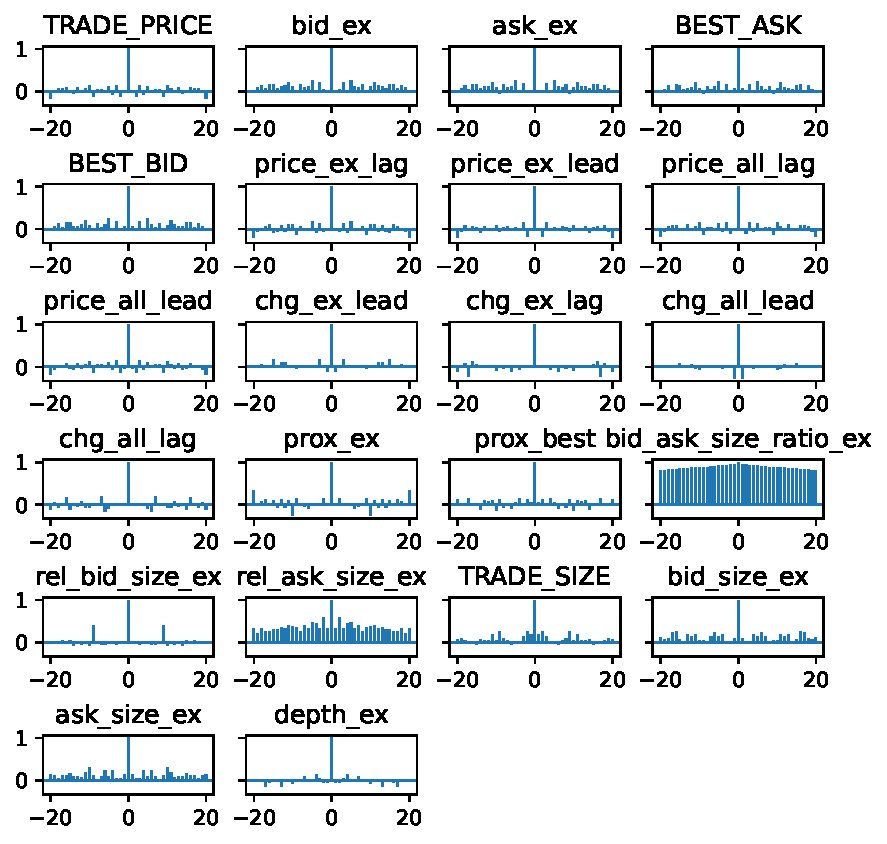
\includegraphics{auto-corr-features.pdf}
    \caption[Autocorrelation of Features]{Autocorrelation Features. Own work.}
    \label{fig:auto-correlation-features}
\end{figure}

\subsection{Results of Hyperparameter Searches}

\begin{table}[H]
    \centering
    \sisetup{table-number-alignment=left}
    \caption[Solutions of Gradient Boosting]{Solutions of gradient boosting. The three right columns document the best combination in terms of validation accuracy per feature set. We perform \num{50} trials each.}
    \label{tab:solutions-gbm}
    \begin{tabular}{@{}llSSS@{}}
        \toprule
        Hyperparameter               & Distribution                                  & {FS 1}              & {FS 2}              & {FS 3}              \\ \midrule
        Depth                        & $\operatorname{UniformInt}[1,12]$             & 8                   & 9                   & 12                  \\
        Learning rate $\eta$         & $\operatorname{LogUniform}[0.001, 0.125]$     & 0.12484221864046671 & 0.12347889459796775 & 0.12471458170177774 \\
        $\ell_2$ Leaf Regularisation & $\operatorname{UniformInt}[2, 30]$            & 15                  & 5                   & 16                  \\
        Random Strength              & $\operatorname{LogUniform}[\num{1e-9}, 10.0]$ & \num{4e-9}          & \num{4e-7}          & \num{8e-6}          \\
        Bagging Temperature          & $\operatorname{Uniform}[0.0, 1.0]$            & 0.6419530220498153  & 0.5574912093427532  & 0.45578836944233    \\ \midrule
        Validation Accuracy in \%    &                                               & 64.37816236230594   & 75.03504680858162   & 76.99459643967347   \\ \bottomrule
    \end{tabular}
\end{table}

\begin{table}[H]
    \centering
    \sisetup{table-number-alignment=left}
    \caption[Hyperparameter Search Space of Gradient Boosting With Self-Training]{Hyperparameter search space of gradient boosting with self-training. The three right columns document the best combination in terms of validation accuracy per feature set. We perform \num{50} trials each. Arrows indicate the change compared to the supervised variant. }
    \label{tab:solutions-gbm-self-training}
    \begin{tabular}{@{}llSSS@{}}
        \toprule
        Hyperparameter             & Distribution  & {FS 1}         & {FS 2}       & {FS 3}       \\ \midrule
        Depth                       &$\operatorname{UniformInt}[1,12]$   & 9              & 10            & 9            \\
        Learning rate $\eta$        &$\operatorname{LogUniform}[0.001, 0.125]$  & 0.12337960608926582              & 0.1248422186404667            & 0.12347504812996231           \\
        $\ell_2$ Leaf Regularisation &$\operatorname{UniformInt}[2, 30]$ & 12              & 9            & 13            \\
        Random Strength             & $\operatorname{LogUniform}[\num{1e-9}, 10.0]$& \num{2e-8}     & \num{5e-8}   & \num{5e-8}   \\
        Bagging Temperature         &$\operatorname{Uniform}[0.0, 1.0]$  &   0.34010535578784745             & 0.5214954412829511            & 0.4666577105566224             \\ \midrule
        Validation Accuracy in \%   & & {$\downarrow \num{64.29671279599335}$} & {$\downarrow \num{74.83010065958079}$} & {$\downarrow \num{76.41433947686962}$} \\ \bottomrule
    \end{tabular}
\end{table}

\begin{table}[H]
    \centering
    \sisetup{table-text-alignment=left}
    \caption[Solutions of Hyperparameter Search Space of FT-Transformer]{Hyperparameter search space of FT-Transformer. The three right columns document the best combination in terms of validation accuracy per feature set. We perform \num{10} trials each. A discussion of these results is provided below.}
    \label{tab:solutions-transformer}
    \begin{tabular}{@{}llSSS@{}}
        \toprule
        Hyperparameter                       & Distribution                                        & {FS 1} & {FS 2} & {FS 3} \\ \midrule
        Layers $L$                           & $\operatorname{UniformInt}[1,6]$                    &        &        &        \\
        Embedding dimension $d_{\mathrm{e}}$ & $\operatorname{UniformInt}[64, 256]$                &        &        &        \\
        Attention dropout                    & $\operatorname{Uniform}[0, 0.5]$                    &        &        &        \\
        \gls{FFN} dropout                    & $\operatorname{Uniform}[0, 0.5]$                    &        &        &        \\
        Learning rate $\eta$                 & $\operatorname{LogUniform}[\num{3e-5}, \num{3e-4}]$ &        &        &        \\
        weight decay $\lambda$               & $\operatorname{LogUniform}[\num{1e-6}, \num{1e-3}]$ &        &        &        \\ \midrule
        Validation Accuracy in \%  &  & {$\downarrow \num{0.0}$} & {$\downarrow \num{0.0}$} & {$\downarrow \num{0.0}$} \\ \bottomrule
    \end{tabular}
\end{table}